\begin{intersong}
    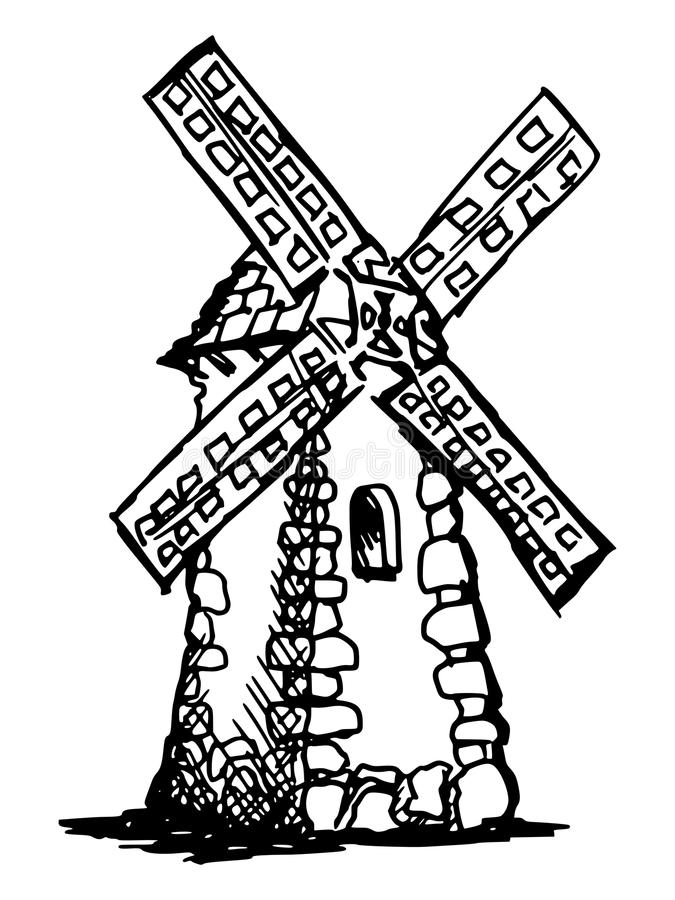
\includegraphics[width=0.4\textwidth]{diemooiemolen}
\end{intersong}
\beginsong{Die mooie molen}
\beginverse
Ik weet een heerlijk plekje grond, alwaar een molen staat,
waar ik mijn allerliefste vond, waarvoor mijn harte slaat.
Ik zag haar voor de eerste keer aan d’oever van de vliet, 
en sinds die tijd kom ik daar weer, die plek vergeet ik niet.
\endverse
\beginchorus
Daar bij die molen, die mooie molen,
daar woont een meisje waar ik zoveel van hou.
Daar bij die molen, die mooie molen,
daar wil ik wonen als jij een wordt mijn vrouw.
\endchorus
\beginverse
Als in de stille avondstond de zon ten onder ging,
en ik haar bij die molen vond in zoete mijmering,
fluisterde zij me in het oor hoe heerlijk saam te zijn.
De molen draaide lustig door en 'k zie “mijn liefste mijn”.
\endverse
\beginverse
Ik zie de molen al versierd ter eer van 't jonge paar,
en heel het dorp dat juicht en viert “zij leven menig jaar”.
En zie ik trots de molen staan, dan zweer ik in die stond,
nooit ga ik van die plek vandaan, waar ik mijn vrouwtje vond.
\endverse
\endsong